\chapter{Versionskontrolle mit Git}

Speziell in großen und komplexen Software-Projekten ist eine gute Versionskontrolle des zu entwickelnden Codes unabdingbar.
Hierfür hat sich Git in den letzten Jahren als Standard entwickelt. Git ist besonders leistungsfähiges und flexibles Versionskontrollwerkzeug mit geringem Aufwand, dass die Entwicklung im Team immens vereinfacht, \cite{Loeliger:2012}.

Hierbei ermöglicht Git das arbeiten in sogenannten \textit{Repositories}. Dies sind einfache Datenbanken, welche alle nötigen Informationen enthält, die für die Aufbewahrung und Verwaltung der Revisionen und des Verlaufs eines Projekts erforderlich sind, \cite{Loeliger:2012}. Hierbei werden zwischen lokalen und remote Repositories unterschieden. Auf das remote Repository kann das gesamte Entwicklungsteam zurück greifen und enthält den aktuellsten Stand der zu entwickelnden Software. Die Entwicklung hingegen erfolgt meistens auf lokalen Repositories, auf welche nur einzelne Entwickler, bzw kleine Entwicklungsteams zugriff haben.

Über den \textbf{clone}- Befehl kann ein Klon des remote Repository im lokalen Repository erzeugt werden.
Weitere wichtige Befehle zum arbeiten mit Repositories sind:
\begin{itemize}
	\item  \textbf{pull}:
	Änderungen aus einem (remote) Repository in das (lokale) Repository übernehmen.
	\item  \textbf{push}:
	Änderungen des (lokalen) Repository in das (remote) Repository hinzufügen.
\end{itemize}

Zentraler Bestandteil der Versions-Kontrolle sind sogenannte \textit{commits}. Werden Änderungen am Code bzw. am Software-Projekt vorgenommen, dann kann einen neue Version über den \textbf{commit}- Befehl erstellt werden. Hierbei werden auch nützliche Informationen wie der Author, Kommentare und eine Commit-Id, sowie alle Änderungen gespeichert. Somit ist zu jedem Zeitpunkt möglich diesen Stand wieder herzustellen.

Weiter ist es möglich, dass mehrere Entwickler parallel an der Entwicklung arbeiten. Hierzu bietet Git das arbeiten in sogenannten Branches. Eine Branche ist eine Abzweigung eines bestimmten Commits und somit einem bestimmten Stand und werden über den \textbf{branch}- Befehl erzeugt. Weitere wichtige Befehle zum Arbeiten mit Branches sind:
\begin{itemize}
	\item  \textbf{chekout}:
	Wechsel in eine andere Branch.
	\item  \textbf{merge}:
	Zwei Branches zu einer Branch zusammenfügen.
\end{itemize}  

In Abbildung \ref{fig:Git} ist beispielhaft ein Git-Projekt dargestellt. Hier sind vier Branches (testing, dev, master, Stabel) sowie mehrere Commits (A - Z) zu sehen.

\begin{figure}[h]
	\centering
	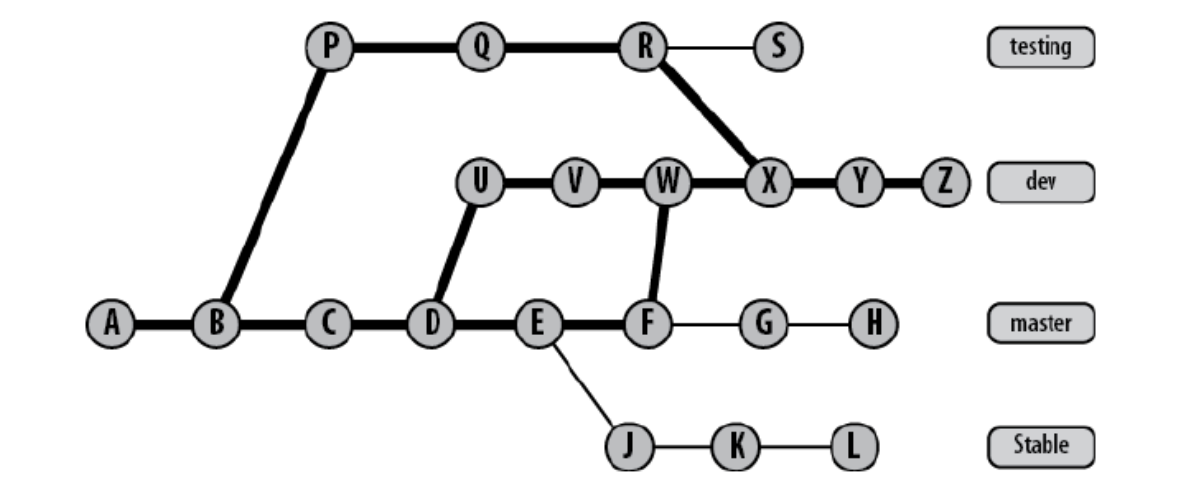
\includegraphics[width=8cm]{pics/Git.png}
	\caption{Branches und Commits, \cite{Loeliger:2012}}
	\label{fig:Git}
\end{figure}  